\documentclass[tikz,border=7pt]{standalone}
\usepackage{amsmath,amssymb}
\usetikzlibrary{arrows.meta,patterns,decorations.markings,calc}
\tikzset{outline/.style={line width=.7pt,line cap=round,line join=round},
 map/.style={outline,-{Stealth[length=2.1mm,width=1.5mm]}},
 point/.style={circle,draw,fill=white,inner sep=1.4pt,line width=.6pt},
 along/.style={postaction={decorate},decoration={markings,mark=at position .52 with {\arrow{Stealth[length=1.8mm,width=1.2mm]}}}}}
\begin{document}
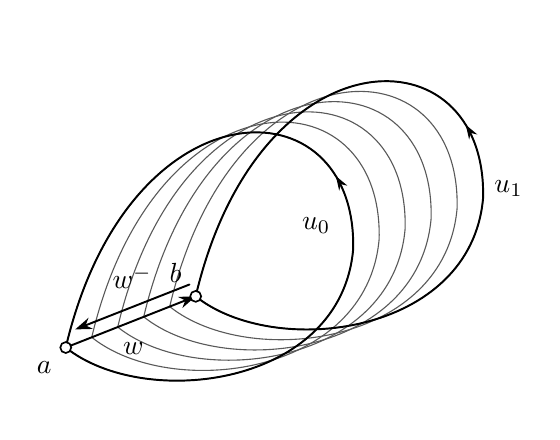
\begin{tikzpicture}[font=\normalsize]

\foreach \s in {0,.2,.4,.6,.8,1}{
\pgfmathsetmacro{\x}{1.65*\s}\pgfmathsetmacro{\y}{.65*\s}
\draw[line width=.4pt,black!65] (\x,\y) .. controls ({\x+1}, {\y-.8}) and ({\x+3.5},{\y-.5}) .. ({\x+3.65},{\y+1.25}) .. controls ({\x+3.7},{\y+3.4}) and ({\x+.8},{\y+3.4}) .. (\x,\y);}
\foreach \s in {0,1}{
\pgfmathsetmacro{\x}{1.65*\s}\pgfmathsetmacro{\y}{.65*\s}
\draw[outline,along] (\x,\y) .. controls ({\x+1}, {\y-.8}) and ({\x+3.5},{\y-.5}) .. ({\x+3.65},{\y+1.25}) .. controls ({\x+3.7},{\y+3.4}) and ({\x+.8},{\y+3.4}) .. (\x,\y);}
\draw[map] (0,0)--(1.65,.65) node[pos=.52,below=4pt] {$w$};
\draw[map] (1.57,.8)--(.12,.23) node[pos=.5,above=3pt] {$w^{-}$};
\node[point,label=below left:$a$] at (0,0) {};
\node[point,label=above left:$b$] at (1.65,.65) {};
\node at (3.18,1.55) {$u_0$};
\node[right] at (5.32,2.02) {$u_1$};

\end{tikzpicture}
\end{document}
